\documentclass[twoside]{article}

%
% This is a borrowed LaTeX template file for lecture notes for CS267,
% Applications of Parallel Computing, UCBerkeley EECS Department.
% Now being used for CMU's 10725 Fall 2012 Optimization course
% taught by Geoff Gordon and Ryan Tibshirani.  When preparing 
% LaTeX notes for this class, please use this template.
%
% To familiarize yourself with this template, the body contains
% some examples of its use.  Look them over.  Then you can
% run LaTeX on this file.  After you have LaTeXed this file then
% you can look over the result either by printing it out with
% dvips or using xdvi. "pdflatex template.tex" should also work.
%

\setlength{\oddsidemargin}{0.25 in}
\setlength{\evensidemargin}{-0.25 in}
\setlength{\topmargin}{-0.6 in}
\setlength{\textwidth}{6.5 in}
\setlength{\textheight}{8.5 in}
\setlength{\headsep}{0.75 in}
\setlength{\parindent}{0 in}
\setlength{\parskip}{0.1 in}

%
% ADD PACKAGES here:
%

\usepackage{amsmath,amsfonts,graphicx}

%
% The following commands set up the lecnum (lecture number)
% counter and make various numbering schemes work relative
% to the lecture number.
%
\newcounter{lecnum}
\renewcommand{\thepage}{\thelecnum-\arabic{page}}
\renewcommand{\thesection}{\thelecnum.\arabic{section}}
\renewcommand{\theequation}{\thelecnum.\arabic{equation}}
\renewcommand{\thefigure}{\thelecnum.\arabic{figure}}
\renewcommand{\thetable}{\thelecnum.\arabic{table}}

%
% The following macro is used to generate the header.
%
\newcommand{\lecture}[4]{
   \pagestyle{myheadings}
   \thispagestyle{plain}
   \newpage
   \setcounter{lecnum}{#1}
   \setcounter{page}{1}
   \noindent
   \begin{center}
   \framebox{
      \vbox{\vspace{2mm}
    \hbox to 6.28in { {\bf Econ 626: Quantitative Methods II
  \hfill Fall 2018} }
       \vspace{4mm}
       \hbox to 6.28in { {\Large \hfill Lecture #1: #2  \hfill} }
       \vspace{2mm}
       \hbox to 6.28in { {\it Lecturer: #3 \hfill Scribes: #4} }
      \vspace{2mm}}
   }
   \end{center}
   \markboth{Lecture #1: #2}{Lecture #1: #2}

   %{\bf Note}: {\it LaTeX template courtesy of UC Berkeley EECS dept.}

   {\bf Disclaimer}: {\it Zhikun is fully responsible for the errors and typos appeared in the notes.}
   \vspace*{4mm}
}
%
% Convention for citations is authors' initials followed by the year.
% For example, to cite a paper by Leighton and Maggs you would type
% \cite{LM89}, and to cite a paper by Strassen you would type \cite{S69}.
% (To avoid bibliography problems, for now we redefine the \cite command.)
% Also commands that create a suitable format for the reference list.
\renewcommand{\cite}[1]{[#1]}
\def\beginrefs{\begin{list}%
        {[\arabic{equation}]}{\usecounter{equation}
         \setlength{\leftmargin}{2.0truecm}\setlength{\labelsep}{0.4truecm}%
         \setlength{\labelwidth}{1.6truecm}}}
\def\endrefs{\end{list}}
\def\bibentry#1{\item[\hbox{[#1]}]}

%Use this command for a figure; it puts a figure in wherever you want it.
%usage: \fig{NUMBER}{SPACE-IN-INCHES}{CAPTION}
\newcommand{\fig}[3]{
      \vspace{#2}
      \begin{center}
      Figure \thelecnum.#1:~#3
      \end{center}
  }
% Use these for theorems, lemmas, proofs, etc.
\newtheorem{theorem}{Theorem}[lecnum]
\newtheorem{lemma}[theorem]{Lemma}
\newtheorem{proposition}[theorem]{Proposition}
\newtheorem{claim}[theorem]{Claim}
\newtheorem{corollary}[theorem]{Corollary}
\newtheorem{definition}[theorem]{Definition}
%\newtheorem{example}[theorem]{Example}
\newenvironment{proof}{{\bf Proof:}}{\hfill\rule{2mm}{2mm}}
\newenvironment{example}{{\bf Example:}}{\hfill\rule{2mm}{2mm}}

\newtheorem{remark}[theorem]{Remark}
%\newenvironment{remark}[1][Remark]{\begin{trivlist}\item[\hskip \labelsep {\bfseries #1}]}{\end{trivlist}}


% **** IF YOU WANT TO DEFINE ADDITIONAL MACROS FOR YOURSELF, PUT THEM HERE:

\newcommand\E{\mathbb{E}}
\newcommand\dd{\mathrm{d}}

\usepackage{hyperref}
\newcommand\pp{\partial}
\usepackage{listings}

\begin{document}
%FILL IN THE RIGHT INFO.
%\lecture{**LECTURE-NUMBER**}{**DATE**}{**LECTURER**}{**SCRIBE**}
\lecture{2}{Dynamic Programming II}{Prof. Daniel Levy}{Zhikun Lu}
%\footnotetext{These notes are partially based on those of Nigel Mansell.}
\footnotetext[1]{Visit \url{http://www.luzk.net/misc} for updates.}

\hfill Date: August 30, 2018

\section{Infinite Horizon Model}
{\bf (Growth Model -- Lucas, Stokey and Prescott)}
\begin{equation}
    V(K_0) = \begin{cases}
        \max\limits_{\{C_0, K_1\}} [u(C_0)+ \beta V(K_1)]\\
        \quad s.t. \quad C_0 + K_1 = f(K_0)
    \end{cases}
\end{equation}
\begin{equation}
    \Longrightarrow V(K_0) = \max\limits_{\{ K_1\}} [u(f(K_0)-K_1)+ \beta V(K_1)]
\end{equation}

\underline{FONC}

\begin{equation}
    u'(f(K_0)-K_1) = \beta V'(K_1)
\end{equation}
By assumption
\begin{equation}
    K_1 = g(K_0)
\end{equation}
\begin{equation}
    V(K_0) = u(f(K_0)-g(K_0)) + \beta V(g(K_0))
\end{equation}
\underline{Total differential}:
\begin{equation}
    \begin{aligned}
        V'(K_0) &= u'(f(K_0)-g(K_0))(f'(K_0) - g'(K_0))+ \beta V'(g(K_0))g'(K_0)\\
        &= u'(f(K_0)-g(K_0))  f'(K_0) - [u'(f(K_0)-g(K_0))- \beta V'(g(K_0)) ]  g'(K_0)\\
        &= u'(f(K_0)-g(K_0))  f'(K_0)
    \end{aligned}
\end{equation}
Here, $[u'(f(K_0)-g(K_0))- \beta V'(g(K_0)) ]  g'(K_0) = 0$ by FONC (2.3), which follows from the envelope theorem.

\underline{Lead one period}
\begin{eqnarray}
    V'(K_1) &=& u'(f(K_1)-K_2)  f'(K_1)\\
    \Longrightarrow u'(f(K_0)-K_1) &=& \beta u'(f(K_1)-K_2)  f'(K_1)
\end{eqnarray}
which is a second order difference equation in $K$.

\underline{Assumptions}
\begin{eqnarray}
    f(K_t) &=& K_t^\alpha, \quad 0 < \alpha < 1\\
    u(C_t) &=& \ln C_t
\end{eqnarray}

\underline{Recall}
\begin{equation}
    V(K_t) = \begin{cases}
        \max\limits_{\{C_t, K_{t+1}\}} [u(C_t)+ \beta V(K_{t+1})]\\
        \quad s.t. \quad C_t + K_{t+1} = f(K_t)
    \end{cases}
\end{equation}

\underline{Choice Variables}: $\{C_t, K_{t+1}\}_{t=0}^{\infty}$

\underline{Set up a Lagrangian}
\begin{equation}
    \mathcal{L} = u(C_t)+ \beta V(K_{t+1}) + \lambda_t [ f(K_t) - C_t - K_{t+1}]
\end{equation}
With our functional forms, it becomes
\begin{equation}
    \mathcal{L} = \ln C_t+ \beta V(K_{t+1}) + \lambda_t [ K_t^\alpha - C_t - K_{t+1}]
\end{equation}

\underline{FONC}
\begin{eqnarray}
    &[C_t]&     \frac{1}{C_t} - \lambda_t = 0\\
    &[K_{t+1}]&  \beta V'(K_{t+1}) - \lambda_t = 0\\
    &\Longrightarrow& \frac{1}{C_t} = \beta V'(K_{t+1})
\end{eqnarray}
Apply the envelope theorem again [\texttt{Benveniste-Scheinkman Theorem}]. Suppose we have a solution of all variables as a function of the state:
\begin{eqnarray}
    C_t &=& C_t(K_t)\\
    K_{t+1} &=& K_{t+1}(K_t)\\
    \lambda_t &=& \lambda_t(K_t)
\end{eqnarray}
then (2.13) $\Longrightarrow$
\begin{equation}
    V(K_t) = \mathcal{L}^* = \ln C_t(K_t) + \beta V(K_{t+1}(K_t)) + \lambda_t(K_{t}) [ K_t^\alpha - C_t(K_t) - K_{t+1}(K_t)]
\end{equation}
which is a function of $K_t$ only.

Differentiate w.r.t. $K_t$
\begin{eqnarray}
    V'(K_t) &=& \frac{1}{C_t(K_t)}C_t'(K_t) + \beta V'(K_{t+1})K_{t+1}'(K_t) + \lambda_t'(K_t) [ K_t^\alpha - C_t(K_t) - K_{t+1}(K_t)] + \lambda_t(K_t) [\alpha K_t^{\alpha-1}- C_t'(K_t) - K_{t+1}'(K_t)]\\
    &=& \frac{1}{C_t(K_t)}C_t'(K_t) + \beta V'(K_{t+1})K_{t+1}'(K_t) + \lambda_t(K_t) [\alpha K_t^{\alpha-1}- C_t'(K_t) + K_{t+1}'(K_t)] \quad (\text{as } K_t^\alpha - C_t - K_{t+1} = 0)\\
    &=& C_t'(K_t) \left [ \frac{1}{C_t(K_t)} - \lambda_t(K_{t}) \right ] + K_{t+1}'(K_t)[\beta V'(K_{t+1}(K_{t})) - \lambda_t(K_t)] + \lambda_t(K_t) \alpha K_t^{\alpha-1}\\
    &=&  \lambda_t(K_t) \alpha K_t^{\alpha-1} \qquad (\text{since the first two terms are 0 by FONC)}\\
    &=& \frac{1}{C_t(K_t)} \alpha K_t^{\alpha-1}
\end{eqnarray}
Lead one period forward
\begin{equation}
    V'(K_{t+1}) = \frac{1}{C_{t+1}(K_{t+1})} \alpha K_{t+1}^{\alpha-1} 
\end{equation}
\underline{Note}: we could obtain the same result directly from (2.12) with envelope theorem. If we take the value function of (2.12)
\begin{equation}
    V(K_t) = \max \{ u(C_t)+ \beta V(K_{t+1}) + \lambda_t [ f(K_t) - C_t - K_{t+1}] \}
\end{equation}
and ignore the dependence of $C_t$ and $K_{t+1}$, because we are at a maximum point, then by the envelope theorem:
\begin{equation}
    V'(K_t) = \lambda_t f'(K_t) \quad {\buildrel \text {lead one-period} \over \Longrightarrow} \quad
    V'(K_{t+1}) = \lambda_{t+1} f'(K_{t+1}),
\end{equation}
which is the same as (2.26) because of (2.14).

Next, (2.26) and (2.16) lead to
\begin{equation}
    \frac{1}{C_t} = \beta \frac{1}{C_{t+1}}\alpha K_{t+1}^{\alpha - 1}
\end{equation}
which is a first order difference equation in $C$. Recall the budget constraint
\begin{equation}
    C_t + K_{t+1} = K_t^\alpha,
\end{equation}
which is a first order difference equation in $K$. 

Note that (2.29) and (2.30) are connected. Together, they form a system of two first order difference equations.
$$\begin{cases} 
    \dfrac{1}{C_t} = \beta \frac{1}{C_{t+1}}\alpha K_{t+1}^{\alpha - 1}\\
    C_t + K_{t+1} = K_t^\alpha
\end{cases}$$


\section{Solution Methods}
Three method for solving dynamic programming problems:
\begin{enumerate}
    \item Policy function iteration
    \item Value function iteration
    \item Guess ``intelligently'' (not easy)
\end{enumerate}
\subsection{Policy Function Iteration}
From (2.29), we have \begin{equation}
    \frac{K_{t+1}}{C_t} = \frac{\alpha \beta}{C_{t+1}}K_{t+1}^\alpha
\end{equation}
(2.30) $\Longrightarrow$
\begin{equation}
    1+ \frac{K_{t+1}}{C_t} = \frac{K_t^\alpha}{C_t}
\end{equation}
Together $\Longrightarrow$
\begin{equation}
    \alpha \beta \frac{K_{t+1}^\alpha}{C_{t+1}} = \frac{K_t^\alpha}{C_t} - 1
\end{equation}
which is a first order difference equation in $\dfrac{K^\alpha}{C}$.

Solve the difference equation by sucessive substitution \underline{forward}:
\begin{eqnarray}
    \frac{K_t^\alpha}{C_t} &=& 1+ \alpha \beta \frac{K_{t+1}^\alpha}{C_{t+1}}\\
    \frac{K_{t+1}^\alpha}{C_{t+1}} &=& 1+ \alpha \beta \frac{K_{t+2}^\alpha}{C_{t+2}}\\
    \frac{K_t^\alpha}{C_t} &=& 1+ \alpha \beta (1+ \alpha \beta \frac{K_{t+2}^\alpha}{C_{t+2}})\\
    \frac{K_t^\alpha}{C_t} &=& 1+ \alpha \beta  + (\alpha \beta)^2 \frac{K_{t+2}^\alpha}{C_{t+2}}\\
    \frac{K_{t+2}^\alpha}{C_{t+2}} &=& 1+ \alpha \beta \frac{K_{t+3}^\alpha}{C_{t+3}}\\
    \frac{K_t^\alpha}{C_t} &=& 1+ \alpha \beta  + (\alpha \beta)^2 (1+ \alpha \beta \frac{K_{t+3}^\alpha}{C_{t+3}})\\
    \frac{K_t^\alpha}{C_t} &=& 1+ \alpha \beta  + (\alpha \beta)^2 + (\alpha \beta)^3 \frac{K_{t+3}^\alpha}{C_{t+3}}    
\end{eqnarray}
Continue substituting forward infinitely many times, we get
\begin{equation}
    \frac{K_t^\alpha}{C_t} = 1+ \alpha \beta  + (\alpha \beta)^2 + (\alpha \beta)^3 + \dots + \lim_{s \to \infty} (\alpha \beta)^{s}\frac{K_{t+s}^\alpha}{C_{t+s}}.
\end{equation}
If $\lim_{s \to \infty} (\alpha \beta)^{s}\frac{K_{t+s}^\alpha}{C_{t+s}} = 0$, then
\begin{equation}
    \frac{K_t^\alpha}{C_t} = \sum_{s=0}^{\infty} (\alpha \beta)^s = \frac{1}{1- \alpha \beta},
\end{equation}
which leads to our policy function
\begin{equation}
    C_t^* = (1- \alpha \beta )K_t^\alpha.
\end{equation}


\underline{Comment}

(2.34) $\Longrightarrow$ after N times substitution
\begin{equation}
    \frac{K_t^\alpha}{C_t} = 1+ \alpha \beta  + (\alpha \beta)^2 + \dots + (\alpha \beta)^N + (\alpha \beta)^{N+1}\frac{K_{t+N+1}^\alpha}{C_{t+N+1}}.
\end{equation}

\underline{Assumption}
\begin{equation}
    \lim_{N \to \infty} (\alpha \beta)^{N+1}\frac{K_{t+N+1}^\alpha}{C_{t+N+1}} = 0.
\end{equation}
As $N \to \infty$, $(\alpha \beta)^{N+1} \to 0$. Therefore by assuming the above limit, we are imposing a limit on how fast $\frac{K_{t+N+1}^\alpha}{C_{t+N+1}}$ grows in the future. Specifically, we require that $\frac{K_{t+N+1}^\alpha}{C_{t+N+1}}$ will not grow as $N \to \infty$ at a rate that exceeds the rate in which $(\alpha \beta)^{N+1} $ shrinks.

(2.43) is the \texttt{consumption function}, where $1- \alpha \beta $ is the MPC.

\underline{Plug into } $C_t + K_{t+1} = K_t^\alpha$:
\begin{equation}
    (1- \alpha \beta )K_t^\alpha + K_{t+1} = K_t^\alpha
\end{equation}
\begin{equation}
    K_{t+1}^* = \alpha \beta K_t^\alpha
\end{equation}
\[
\Longrightarrow \frac{K_{t+1}^*}{K_t^\alpha} = \alpha \beta
\]
confirming our assertion that the steady state saving rate is $\alpha \beta $. Thus, (2.43) abd (2.47) are the optimal policy functions.

\subsection{Guess a ``solution"}
Sometimes, based on our experience, we may be able to tell something about the properties of the policy functions.

\underline{For example}

Suppose that we can guess that \begin{equation}
    \frac{K_{t+1}}{K_t^\alpha} = \text{constant} \equiv \Gamma,
\end{equation}
but we don't know its value. Then 
\begin{equation}
    K_{t+1} = \Gamma K_t^\alpha
\end{equation}
\begin{equation}
    C_t = (1-\Gamma) K_t^\alpha
\end{equation}
\begin{equation}
    \frac{K_{t+1}}{C_t} = \frac{\Gamma}{1- \Gamma}
\end{equation}
From (2.31),
\begin{equation}
    \frac{\Gamma}{1- \Gamma} = \frac{K_{t+1}}{C_t} = \frac{\alpha \beta}{C_{t+1}}K_{t+1}^\alpha \Longrightarrow C_{t+1} = \frac{1- \Gamma}{\Gamma}\alpha \beta K_{t+1}^\alpha
\end{equation}
(2.50) $\Longrightarrow$ 
\begin{equation}
    C_{t+1} = (1-\Gamma) K_{t+1}^\alpha
\end{equation}
Comparing (2.52) and (2.53), we conclude that 
\begin{equation}
    \frac{1- \Gamma}{\Gamma}\alpha \beta = 1-\Gamma
\end{equation}
\begin{equation}
    \Gamma = \alpha \beta
\end{equation}

\subsection{Value function iteration}
Value function changes from iteration to iteration, i.e., every period, until convergence.

Typically, we start with some initial functional form, often as simple as $V(\cdot) = 0$, and iterate, until convergence.

\begin{figure}[htbp] 
    \centering
    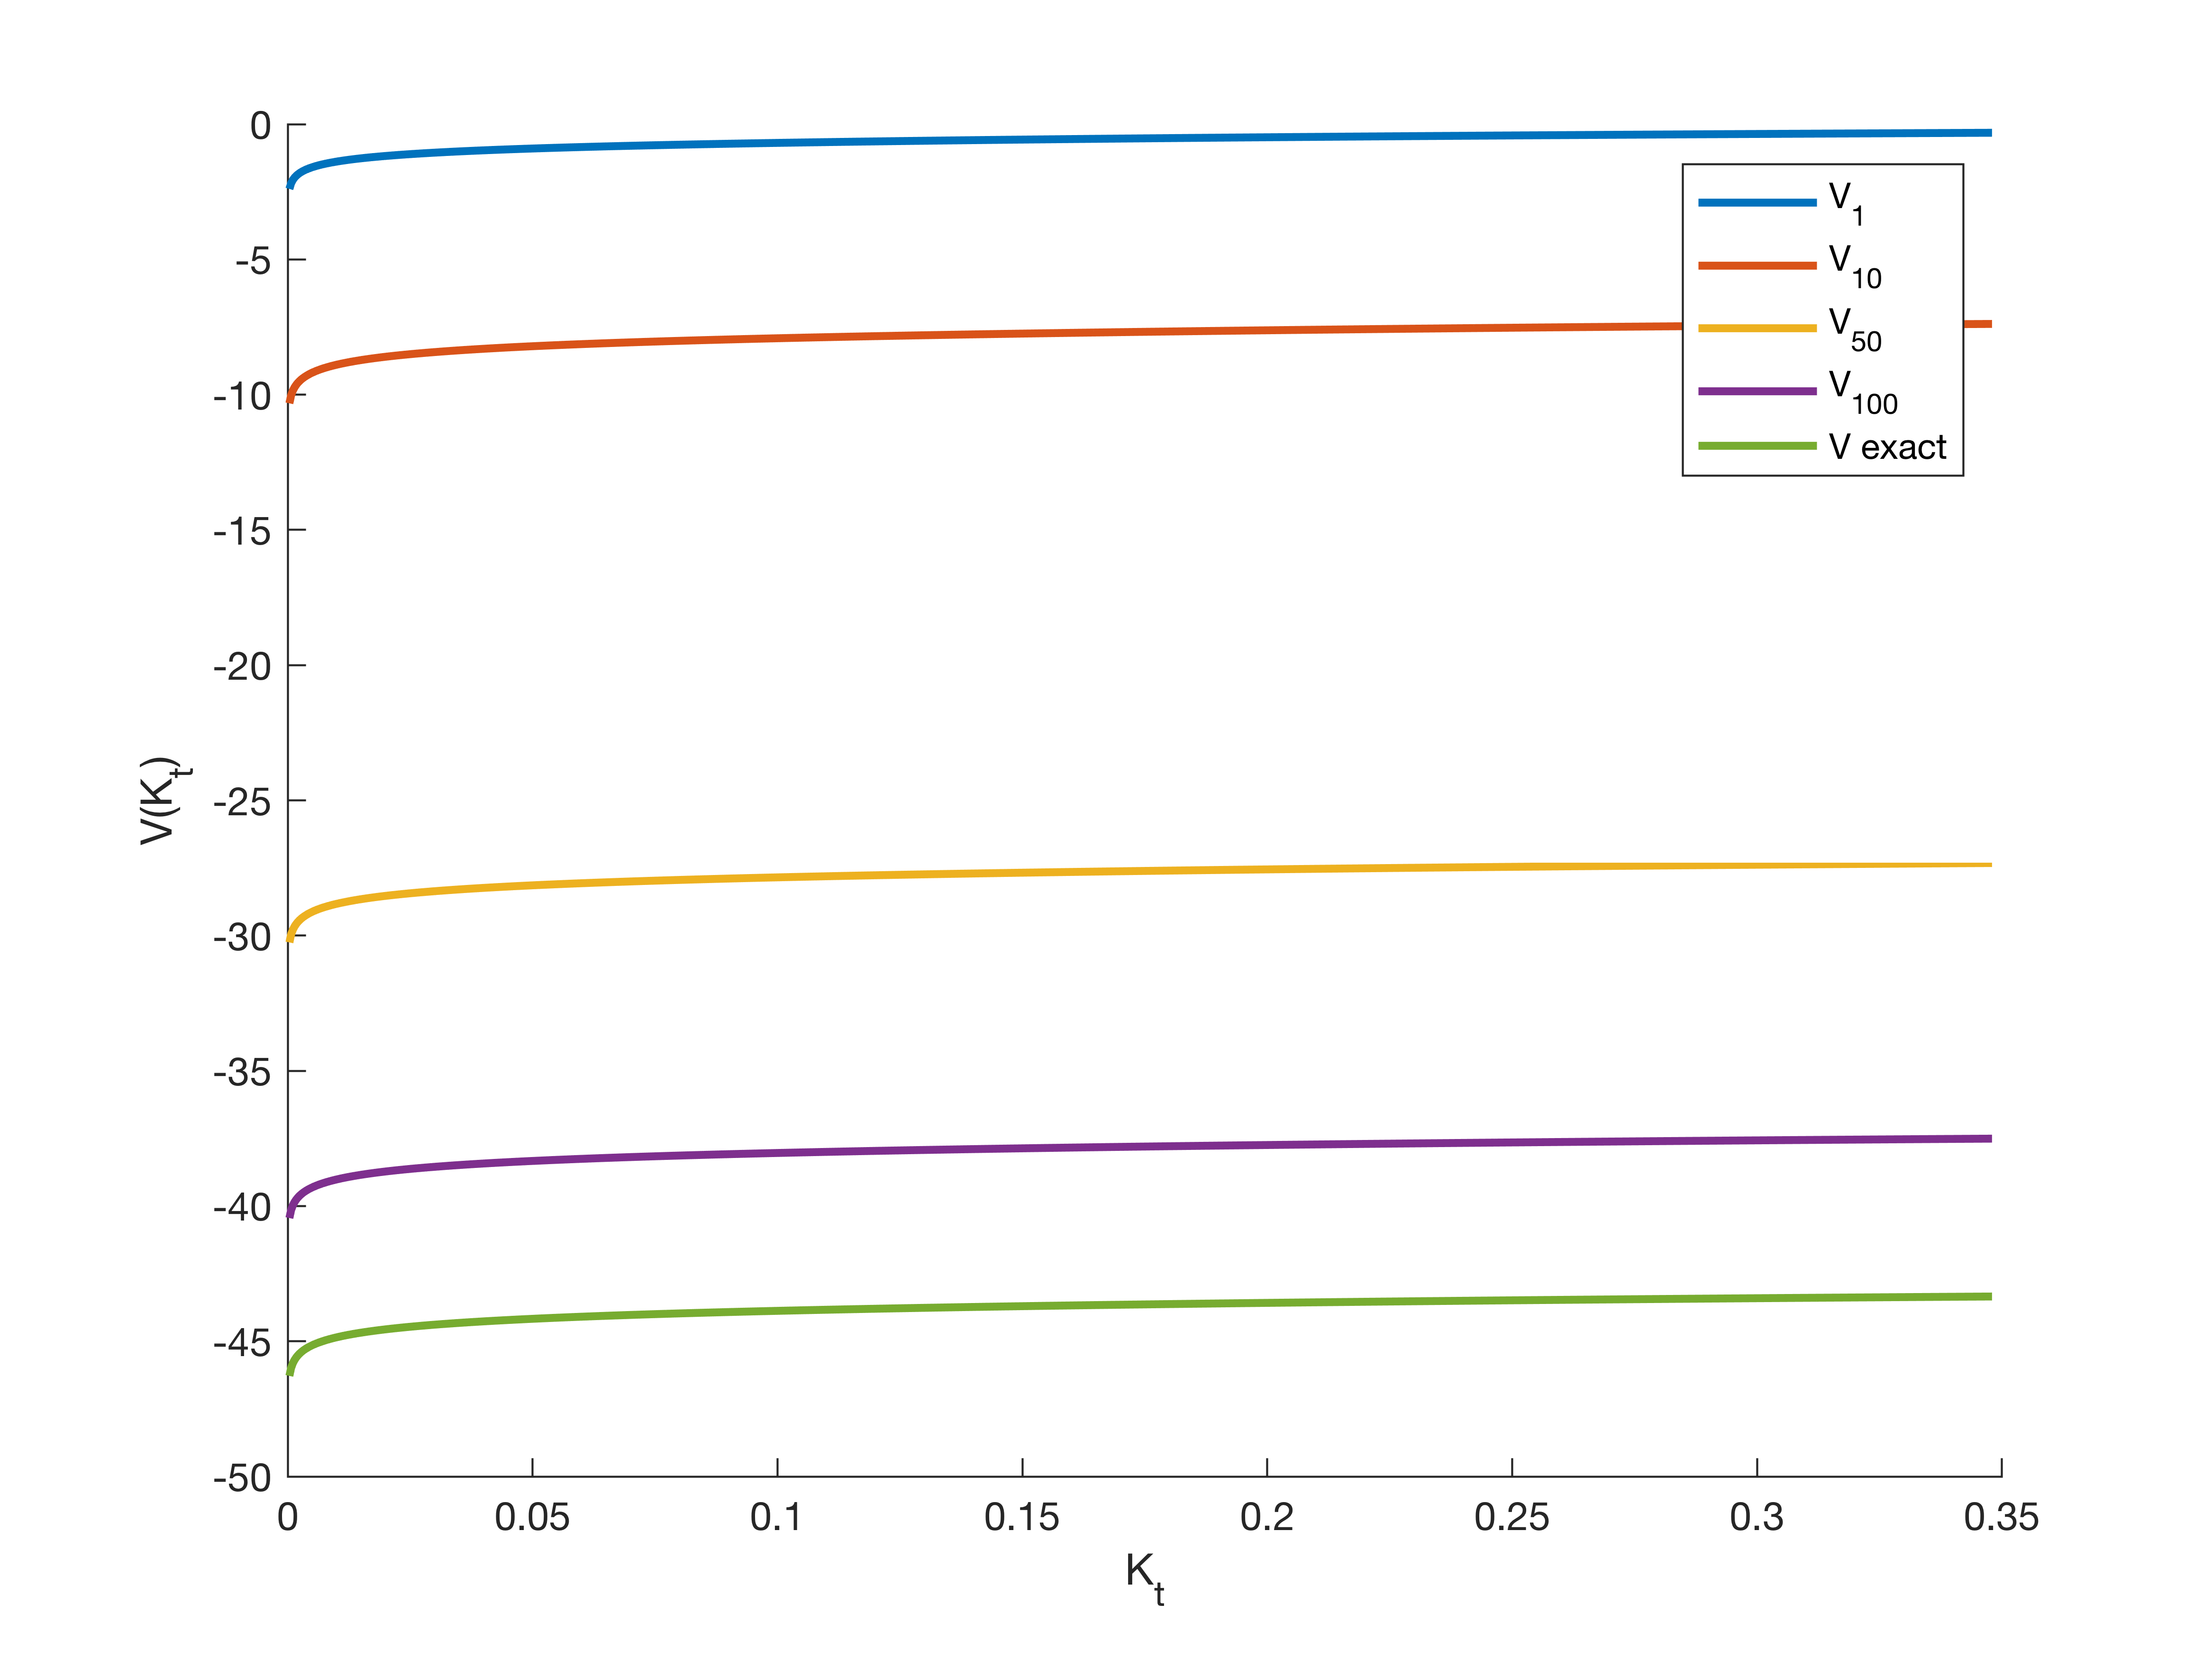
\includegraphics[width=.8\textwidth]{figure/vfi.png}
    %\includegraphics[width=2in]{XeTeX-2.jpg} 
    \caption{An Numerical Example with $\alpha = 0.3, \beta = 0.98$}
\end{figure}

Start with inital guess $V_0(K_{T+1}) = 0$
\begin{equation}
    V_1(K_T) = \begin{cases}
        \max\limits_{\{C_T, K_{T+1}\}} [u(C_T)+ \beta V_0(K_{T+1})]\\
        \quad s.t. \quad C_T + K_{T+1} = K_T^\alpha
    \end{cases}
\end{equation}
\begin{equation}
    \Longrightarrow \begin{cases}
        K_{T+1} = 0\\
        C_T =  K_T^\alpha
    \end{cases}, 
\end{equation}
Hence, $V_1(K_T) = \ln (K_T^\alpha)$. Let's continue:
\begin{equation}
    V_2(K_{T-1}) = \begin{cases}
        \max\limits_{\{C_{T-1}, K_{T}\}} [u(C_{T-1})+ \beta V_1(K_{T})]\\
        \quad s.t. \quad C_{T-1} + K_{T} = K_{T-1}^\alpha
    \end{cases}
\end{equation}
\begin{equation}
    \Longrightarrow V_2(K_{T-1}) = \begin{cases}
        \max\limits_{\{C_{T-1}, K_{T}\}} \ln(C_{T-1})+ \beta \ln (K_T^\alpha)\\
        \quad s.t. \quad C_{T-1} + K_{T} = K_{T-1}^\alpha
    \end{cases}
\end{equation}



Code to reproduce figure (2.1)
\begin{lstlisting}
    clear all;clc;
    % luzhikun
    beta = 0.98; alpha = 0.3; delta = 1;

    f_ss = @(k)alpha*k^(alpha-1)+1-delta-1/beta
    k_ss = fsolve(f_ss,1)
    k_initial = 0.5*k_ss

    num_state = 1000;
    phi = 2*k_ss/num_state;
    k_state = phi:phi:(2*k_ss);

    [K_x, K_y] = meshgrid(k_state,k_state);

    v = zeros(1,num_state);
    epsilon = 10^(-20)

    num_iter = 100

    xx = [1, 10, 50, 100]
    figure(1)
    hold on 
    for ii = 1:num_iter
      v_primitive = v;
      c =  max( K_x.^alpha + (1 - delta)*K_x - K_y, epsilon);
      v_matrix =  log( c ) + beta*v'*ones(1,num_state);
      [v_improved, k_choice_vector] = max(v_matrix);
      v = v_improved;
      %error_ = max(v_improved - v_primitive)
      if (ii == xx(1))|(ii == xx(2))|(ii == xx(3))|(ii == xx(4))
        plot(k_state, v, 'linewidth', 2)
      end
    end

    % exact solution
    v_exact = v;
    a = 1/(1-beta)*(log(1-alpha*beta)+alpha*beta/(1-alpha*beta)*log(alpha*beta));
    b = alpha/(1-alpha*beta);
    v_exact = a+b*log(k_state);
    plot(k_state, v_exact, 'linewidth', 2)

    hold off

    %title('Value function iteration'); 
    xlabel('K_t'); ylabel('V(K_t)');
    legend('V_1', 'V_{10}', 'V_{50}', 'V_{100}','V exact')
\end{lstlisting}






















































































%$$##
\clearpage
\section*{References}
%\beginrefs
%\bibentry{CW87}{\sc D.~Coppersmith} and {\sc S.~Winograd}, 
%``Matrix multiplication via arithmetic progressions,''
%{\it Proceedings of the 19th ACM Symposium on Theory of %Computing},
%1987, pp.~1--6.
%\endrefs

% **** THIS ENDS THE EXAMPLES. DON'T DELETE THE FOLLOWING LINE:

\end{document}


